\documentclass[12pt]{article}
\usepackage[utf8]{inputenc}
\usepackage[T1]{fontenc}
\usepackage{amsmath}
\usepackage{amsfonts}
\usepackage{amssymb}
\usepackage[version=4]{mhchem}
\usepackage{stmaryrd}
\usepackage{graphicx}
\usepackage{chemformula}
\graphicspath{ {./images/} }

\usepackage{listings} % Required for insertion of code
\usepackage{xcolor} % Required for custom colors

% Define custom colors
\definecolor{codegreen}{rgb}{0,0.6,0}
\definecolor{codegray}{rgb}{0.5,0.5,0.5}
\definecolor{codepurple}{rgb}{0.58,0,0.82}
\definecolor{backcolour}{rgb}{0.95,0.95,0.92}

% Setup the style for code listings
\lstdefinestyle{mystyle}{
    backgroundcolor=\color{backcolour},   
    commentstyle=\color{codegreen},
    keywordstyle=\color{magenta},
    numberstyle=\tiny\color{codegray},
    stringstyle=\color{codepurple},
    basicstyle=\ttfamily\footnotesize,
    breakatwhitespace=false,         
    breaklines=true,                 
    captionpos=b,                    
    keepspaces=true,                 
    numbers=left,                    
    numbersep=5pt,                  
    showspaces=false,                
    showstringspaces=false,
    showtabs=false,                  
    tabsize=2
}

% Activate the style
\lstset{style=mystyle}


\title{Chemistry 14 (Spring term 2024) \\
 Midterm Examination }


\author{Distributed Thursday, May 2, 2024\\
Due $\quad$ Thursday, May 9, 2024 by 11:59 pm uploaded through Canvas}
\date{}


\begin{document}
\maketitle


\section*{Conditions}
\begin{itemize}
  \item Open the midterm examination pdf when you are ready to take it.

  \item You have 4 hours to complete this examination (excluding a short break).

  \item You may use the Ch14 online lecture notes, problem sets and solutions, the course web site and a calculator. You may also use the Harris \& Lucy text (or earlier editions). You may also use handwritten notes you have made from other books. You may not discuss the exam with others, use any other books (including those on Reserve), or other web sites.

  \item You may use Mathematica $®$, Matlab®, Excel® or equivalent program to get numerical solutions, including solving polynomial equations. Please note, though, that the problems can be worked with a quadratic equation as the most complex equation that needs to be solved.

  \item Write your answers in the same sequential order as in the exam.

  \item After you have finished the exam, upload your answers through Canvas, just as you do for the problem sets.

  \item Show your work! Getting the right answer is not enough - the intermediate steps are needed for credit. If you use Mathematica $\circledR$ or related program to get numerical solutions, be sure to clearly write out in the exam the specific equation being solved. Note: you do not need to derive equations that were derived in class.

  \item Unless otherwise instructed, you should report answers to 3 significant figures and assume that activities can be approximated by concentrations. You may use approximate formulas as long as you justify the particular approximation (ie in a sufficiently acidic solution, $\left(\mathrm{OH}^{-}\right)$may be neglected relative to $\left(\mathrm{H}^{+}\right)$, etc).

\end{itemize}

\section*{unless otherwise stated, you may assume:}
aqueous solutions

$\mathrm{T}=298.15 \mathrm{~K}=25^{\circ} \mathrm{C}$

$P=1$ atm

$R=8.3144 \mathrm{~J} \mathrm{~mol}^{-1} \mathrm{~K}^{-1}=0.08206$ liter atm $\mathrm{mol}^{-1} \mathrm{~K}^{-1}$

$\mathrm{K}_{w}=10^{-14}$

Debye-Huckel limiting expression, water, $25^{\circ} \mathrm{C}$

individual ionic activity coefficient $\log \gamma_{i}=-0.509 z_{i}^{2} \sqrt{I}$

mean ionic activity coefficient $\quad \log \gamma_{ \pm}=-0.509\left|z_{+} z_{-}\right| \sqrt{I}$

\section*{Chemistry 14 (Spring term 2024)}
Midterm Examination

\begin{center}
\begin{tabular}{lrl}
problem & points &  \\
1a & 5 &  \\
1b & 5 & $\square$ \\
2a & 10 &  \\
$2 b$ & 10 & $\square$ \\
3a & 5 &  \\
3b & 10 & $\square$ \\
3c & 10 & $\square$ \\
3d & 10 & $\square$ \\
3e & 10 & $\square$ \\
4a & 10 &  \\
4b & 10 & $\square$ \\
5 & 5 &  \\
 &  &  \\
total & 100 &  \\
\end{tabular}
\end{center}

\section{Strong acids and strong bases}
Nitric acid is a strong acid and barium hydroxide is a strong base. Assume activities equal concentrations in this problem.

\subsection{}
Calculate the $\mathrm{pH}$ of solution containing $0.001 \mathrm{M}$ barium hydroxide $\left(\mathrm{Ba}(\mathrm{OH})_{2}\right)$.
\subsubsection{Answer}
\begin{align*}
  \ce{Ba(OH)2 &-> Ba^2+ + 2OH-} \\
  \ce{[Ba(OH)2] & = 0.001 M} -> \ce [OH-] = 0.002 M \\
  \ce{Kw & = [H+][OH-]} = 10^{-14} \\
  \ce{[H+] & = \frac{10^{-14}}{0.002}} = 5 \times 10^{-12} \\
  \ce{pH & = -\log[H+]} = 11.3
\end{align*}

\subsection{}

Calculate the $\mathrm{pH}$ of a solution containing $0.1 \mathrm{M}$ barium nitrate $\left(\mathrm{Ba}\left(\mathrm{NO}_{3}\right)_{2}\right)$.
\subsubsection{Answer}
$\left(\mathrm{Ba}\left(\mathrm{NO}_{3}\right)_{2}\right)$ is a salt of a strong acid and a strong base, so it will not affect the $\mathrm{pH}$ of the solution. The $\mathrm{pH}$ of the solution will be the same as the $\mathrm{pH}$ of the water, which is 7.

\section{Weak acids and weak bases}
\subsection{}
Sulfuric acid completely dissociates to $\mathrm{H}^{+}$and $\mathrm{HSO}_{4}^{-}$in solutions more dilute than $0.1 \mathrm{M} . \mathrm{HSO}_{4}$ - further dissociates to $\mathrm{H}^{+}$and $\mathrm{SO}_{4}{ }^{2-}$ with $\mathrm{K}_{\mathrm{a}}=1.02 \times 10^{-2}$. Calculate the $\mathrm{pH}$ of a $0.05 \mathrm{M}$ solution of sulfuric acid. Since sulfuric acid is both a strong acid and a weak acid, start with the charge balance equation for this system. Assume activities equal concentrations.
\subsubsection{Answer}
We are interested in the two dissociation expressions for sulfuric acid:
\begin{align*}
  \ce{H2SO4 &-> H+ + HSO4-} with Ka = \infty \\
  \ce{HSO4- &-> H+ + SO4^2-} with Ka = 1.02 \times 10^{-2}
\end{align*}
We initially know that the concentration of protons is equal to the concentration of sulfuric acid, so $[H+] = 0.05 M$ and $[HSO4-] = 0.05 M$. We can then use the second dissociation to find the concentration of $[SO4^2-]$:
\begin{align*}
  \ce{HSO4- &-> H+ + SO4^2-} \\
  \ce{Ka & = \frac{[H+][SO4^2-]}{[HSO4-]}} \\
\end{align*}
Let us set the parameter $x$ to be the concentration of $[SO4^2-]$. Than the final concentration of $[HSO4-]$ will be $0.05 - x$ and the final concentration of $[H+]$ will be $0.05 + x$. We can then solve for $x$. This suggests the expression:
\begin{align*}
  1.02 \times 10^{-2} & = \frac{(0.05 + x)x}{0.05 - x} \\
\end{align*}
Solving gives a solution for $x$ as 0.00753 M. This means that the concentration of $[H+]$ is $0.05 + 0.00753 = 0.05753 M$. The $\mathrm{pH}$ is then $-\log(0.05753) = 1.24$.
% Inline Python code in the document
\begin{lstlisting}[language=Python]
from sympy import symbols, Eq, solve

# Define the variable
x = symbols('x', real=True, positive=True)

# Given constants
Ka2 = 1.02e-2
initial_H2SO4 = 0.05  # Initial concentration of H2SO4 and hence HSO4-

# Ka expression for the second dissociation of HSO4-
equation_Ka = Eq((initial_H2SO4 + x) * x / (initial_H2SO4 - x), Ka2)

# Solve the equation
x_value = solve(equation_Ka, x)
x_value
\end{lstlisting}
\subsection{}
Calculate the $\mathrm{pH}$ and the equilibrium concentrations of $\left(\mathrm{NH}_{3}\right)$ and $\left(\mathrm{NH}_{4}{ }^{+}\right)$ present in a solution of $\mathrm{NH}_{3}$ made to a total concentration of $1.0 \times 10^{-6} \mathrm{M}\left(=\left(\mathrm{NH}_{3}\right)+\right.$ $\left(\mathrm{NH}_{4}+\right.$ )). The $\mathrm{pK}_{b}$ of $\mathrm{NH}_{3}=4.75$. Assume activities equal concentrations. Although this is a dilute $\mathrm{NH}_{3}$ solution, you can reasonably neglect $\left(\mathrm{H}^{+}\right)$in the charge balance equation.
\subsubsection{Answer}
We are interested in the expression for the equilibrium of $\ce{NH3}$ in water:
\begin{align*}
  \ce{NH3 &-> NH4+ + OH-} \\
  \ce{Kb & = \frac{[NH4+][OH-]}{[NH3]}} \\
\end{align*}
We know the pKb of $\ce{NH3}$ is 4.75, so the Kb is $10^{-4.75}$. The relevant variables that we want to set up is the parameter $x$ to be the concentration of $[OH-]$ and $[NH4+]$ which will be present in equal amounts. If we were to set up a charge balance equation for this process, it would reflect this fact. The final concentration of $[NH3]$ will be $1.0 \times 10^{-6} - x$. This suggests the expression:
\begin{align*}
  10^{-4.75} & = \frac{x^2}{1.0 \times 10^{-6} - x} \\
\end{align*}
Solving for $x$ gives a value of 9.49 $\times 10^{-7} M$.
% Inline Python code in the document
\begin{lstlisting}[language=Python]
from sympy import symbols, Eq, solve, log

# Define the variable
x = symbols('x', real=True, positive=True)

# Given constants
Kb = 10**(-4.75)
initial_NH3 = 1.0e-6  # Total initial concentration of NH3

# Kb expression for the reaction
equation_Kb = Eq(x**2 / (initial_NH3 - x), Kb)

# Solve the equation for x
x_value = solve(equation_Kb, x)
x_value
\end{lstlisting}
So the equilibrium concentrations of $\left(\mathrm{NH}_{4}{ }^{+}\right)$ is $9.49 \times 10^{-7} M$. And that of $\left(\mathrm{NH}_{3}\right)$ is $1.0 \times 10^{-6} - 9.49 \times 10^{-7} = 0.51 \times 10^{-7} M$. The $\mathrm{pOH}$ is $-\log(9.49 \times 10^{-7}) = 6.02$ and the $\mathrm{pH}$ is $14 - 6.02 = 7.98$.






\section{Maintaining a buffer}
\subsection{}
The titration curve of glycine was discussed in lecture 8. The pKa's of glycine are $\mathrm{pK}_{1}=2.35$ and $\mathrm{pK}_{2}=9.78$, respectively. Is glycine a better buffer when $\mathrm{pH}=$ $\mathrm{pK}_{1}$ or when the $\mathrm{pH}$ equals the isoelectric point ( $\mathrm{pl}$ ) of glycine? Explain briefly.
\subsubsection{Answer}
We are given in the lecture that at the isoelectric point, the $[H^+] = \sqrt{K_1K_2}$. This translates to an averaged out pH of 6.07, and is the point where it is in the zwitterionic form. The lecture notes also give that the better buffer exist when the pH is closer to the pKa values. When this is the case, the glycine has a better chance to both accept and donate protons, and hence act as a better buffer. This means that glycine is a better buffer when the pH equals the pKa values of glycine, in this case, when the pH equals $\mathrm{pK}_{1}$.

\subsection{}


What are the fractions of glycine with 0, 1, and 2 protons bound in a solution of glycine when $\mathrm{pH}=\mathrm{pK}_{2}$? Assume activities equal concentrations.
\subsubsection{Answer}
We are interested in the quantity:
\begin{equation}
  \bar{h} = \frac{K_1 [H^+] + 2K_1K_2}{[H^+]^2 + K_1[H^+] + K_1K_2}
\end{equation}
We know that the pH is equal to the pK2, so the concentration of protons is equal to $10^{-9.78}$. We can then substitute this value into the equation.

As given in the lecture, the fractions of each form of glycine are given by:
\begin{align*}
  f_{\ch{H2A+}} &= \frac{[H^+]^2}{[H^+]^2 + K_1 [H^+] + K_1 K_2}, \\
  f_{\ch{HA}} &= \frac{K_1 [H^+]}{[H^+]^2 + K_1 [H^+] + K_1 K_2}, \\
  f_{\ch{A-}} &= \frac{K_1 K_2}{[H^+]^2 + K_1 [H^+] + K_1 K_2}.
\end{align*}

Because the last two fractions are the same, they give values of 0.5 and then because the K2 = $[H^+]$ is much smaller than the K1, the fraction of glycine with 0 protons is much smaller so we can approximate it as 0. The fractions of glycine with 0, 1, and 2 protons bound are 0, 0.5, and 0.5, respectively.
% Inline Python code in the document
\begin{lstlisting}[language=Python]
import math

# Constants
pK1 = 2.35
pK2 = 9.78

# Equilibrium constants
K1 = 10**(-pK1)
K2 = 10**(-pK2)

# Proton concentration at pH = pK2
H_plus = 10**(-pK2)

# Fractions of each form of glycine
f_H2A_plus = H_plus**2 / (H_plus**2 + K1 * H_plus + K1 * K2)
f_HA = K1 * H_plus / (H_plus**2 + K1 * H_plus + K1 * K2)
f_A_minus = K1 * K2 / (H_plus**2 + K1 * H_plus + K1 * K2)

print(f"Fraction of H2A+ (glycine with 2 protons): {f_H2A_plus:.4f}")
print(f"Fraction of HA (glycine with 1 proton): {f_HA:.4f}")
print(f"Fraction of A- (glycine with 0 protons): {f_A_minus:.4f}")
\end{lstlisting}
\subsection{}


What are the concentrations of $\mathrm{HAc}$ and $\mathrm{Ac}^{-}$ in a $0.1 \mathrm{M}$ acetate buffer (i.e., $\left[\mathrm{HAc}\right]+\left[\mathrm{Ac}^{-}\right]=0.1 \mathrm{M}$) at $\mathrm{pH} 4.76$? The $\mathrm{p}K_a$ of $\mathrm{HAc}$ is 4.76. Assume activities equal concentrations.
\subsubsection{Answer}
The relevant equation for this equilibrium process is:
\begin{equation}
  K_a = \frac{[\mathrm{H}^+][\mathrm{Ac}^-]}{[\mathrm{HAc}]}
\end{equation}
We are given the pH, which implies a proton concentration of $[\mathrm{H}^+] = 10^{-4.76}$. This is the same value as the $K_a$. Since the total mass of the buffer must be conserved, we can define $[\mathrm{HAc}] = x \rightarrow [\mathrm{Ac}^-] = 0.1 - x$. We can then substitute these values into the equation and solve for $x$. That script gives a value of 0.05 M for $[\mathrm{HAc}]$ and 0.05 M for $[\mathrm{Ac}^-]$.
% Inline Python code in the document
\begin{lstlisting}[language=Python]
from sympy import symbols, Eq, solve

# Define the variable
x = symbols('x')

# Given constants
total_concentration = 0.1  # Total concentration of HAc + Ac-
pH = 4.76
Ka = 10**(-pH)  # Ka equals [H+] at pH 4.76

# Set up the equation from the given relationship
equation = Eq(Ka * x / (total_concentration - x), Ka)

# Solve the equation
concentration_HAc = solve(equation, x)
concentration_Ac_minus = total_concentration - concentration_HAc[0]

concentration_HAc, concentration_Ac_minus

\end{lstlisting}
\subsection{}

Calculate the volumes of glacial acetic acid (17.4 M) and $2.54 \mathrm{M} \mathrm{NaOH}$ needed to make 2 liters of $0.2 \mathrm{M}$ acetate buffer, pH 5.0 (i.e., $(\mathrm{HAc})+(\mathrm{Ac}^{-})=0.2 M$). Assume activities equal concentrations.
\subsubsection{Answer}
Let us use the Henderson-Hasselbalch equation to solve this problem. The equation is given by:
\begin{equation}
  \mathrm{pH} = \mathrm{p}K_{a}+\log \left(\frac{[\mathrm{Ac}^{-}]}{[\mathrm{HAc}]}\right)
\end{equation}
In the previous part of the problem, we are given that the pKa of HAc is 4.76 and then we know that the pH is 5.0. So, the equation simplifies to:
\begin{equation}
  0.24 = \log \left(\frac{[\mathrm{Ac}^{-}]}{[\mathrm{HAc}]}\right)
\end{equation}
This allows us to compute the ratio $[\mathrm{Ac}^{-}] / [\mathrm{HAc}]$. If we set $x$ to be the number of moles of HAc, the total number of moles is 2 liters * 0.2 M = 0.4 moles. This gives us the relation $[\text{moles}_{\mathrm{Ac}^{-}}] = 0.4 - x$. We can then substitute these values into the equation and solve for $x$. Then it is straightforward to solve for the volumes needed, as we can use the definition of molarity:
\begin{equation}
  \text { Molarity }=\frac{\text { moles solute }}{\text { liters solution }}
\end{equation}
That script gives a value of 8.40 mL for the volume of glacial acetic acid and 100. mL for the volume of $2.54 M \mathrm{NaOH}$.
% Inline Python code in the document
\begin{lstlisting}[language=Python]
import math
from sympy import symbols, Eq, solve

# Define the variable
x = symbols('x', positive=True, real=True)

# Given data
pH = 5.0
pKa = 4.76
total_concentration = 0.2  # M
total_volume = 2  # liters of solution
conc_acetic_acid = 17.4  # M
conc_NaOH = 2.54  # M

# Calculate the ratio from the Henderson-Hasselbalch equation
ratio_Ac_minus_to_HAc = 10**(pH - pKa)

# Total moles in solution
total_moles = total_concentration * total_volume  # 0.4 moles

# Equation for moles of HAc
equation = Eq(x + ratio_Ac_minus_to_HAc * x, total_moles)

# Solve for x
moles_HAc = solve(equation, x)[0]
moles_Ac_minus = ratio_Ac_minus_to_HAc * moles_HAc

# Calculate volumes needed for each component
volume_HAc = moles_HAc / conc_acetic_acid
volume_NaOH = moles_Ac_minus / conc_NaOH

volume_HAc, volume_NaOH

\end{lstlisting}

\subsection{}
A citrate buffer is made up of $0.01 \mathrm{M} \mathrm{Na}_{2} \mathrm{H}$ citrate and $0.01 \mathrm{M} \mathrm{Na}_{3}$ citrate, where the relevant $\mathrm{pK}_{3}=6.40$ for this reaction:

$$
\text { Hcitrate }^{2-} \stackrel{K_{3}}{\rightleftharpoons} \text { citrate }^{3-}+H^{+}
$$

Using the Debye-Huckel limiting law and the Henderson-Hasselbalch equation, estimate the actual $\mathrm{pH}$ of this buffer. You can neglect the contribution of $\mathrm{H}+$ and $\mathrm{OH}-$ to the ionic strength.

(citrate is a tricarboxylic acid with the following structure:

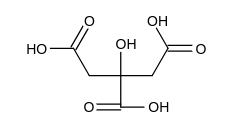
\includegraphics{smile-lvslvvf9smi5kvdw2w.png}


Hcitrate ${ }^{2-}$ and citrate ${ }^{3-}$ have 2 and 3 dissociated protons, respectively.)
\subsubsection{Answer}
The Henderson-Hasselbalch equation is given by:
\begin{equation}
  \mathrm{pH} = \mathrm{p}K_{a}+\log \left(\frac{[\text { citrate }^{3-}]}{[\text { Hcitrate }^{2-}]}\right)
\end{equation}
so since we know that the concentrations what be the same, in the ideal case pH = pKa. However, we are asked to estimate the actual pH of the buffer,which will be mortified by the activities. The Debye-Huckel limiting law is given by:
\begin{equation}
  \log \gamma_{\pm}=-0.509\left|z_{+} z_{-}\right| \sqrt{I}
\end{equation}
where $I$ is the ionic strength of the solution. The ionic strength is given by:
\begin{equation}
  I = \frac{1}{2} \sum_{i} m_{i} z_{i}^{2}
\end{equation}
where $m_{i}$ is the molarity of the ion and $z_{i}$ is the charge of the ion. The ionic strength is then given by:
\begin{equation}
  I = \frac{1}{2} \left(0.01 \times 2^{2} + 0.01 \times 3^{2}\right) = 0.065
\end{equation}
We can then use the Debye-Huckel limiting law to estimate the activity coefficients of the ions as $\gamma_{\text {citrate }}=0.0679$ and $\gamma_{\text {Hcitrate }}= 0.303$.
This means  that the actual concentrations that enter into the Henderson-Hasselbalch equation are $0.01 \times 0.0679$ and $0.01 \times 0.303$. The actual pH of the buffer is then $6.40 + \log(0.01 \times 0.0679 / 0.01 \times 0.303) = 5.75$.

% Inline Python code in the document
% Inline Python code in the document
\begin{lstlisting}[language=Python]

import math
# Constants and values from the problem statement
pKa = 6.40
concentration_Hcitrate = 0.01  # M
concentration_citrate = 0.01  # M
ionic_strength = 0.065  # calculated in the problem statement

# Constants for Debye-Huckel equation
A = 0.509
z_citrate = 3
z_Hcitrate = 2

# Calculating activity coefficients using Debye-Huckel limiting law
gamma_citrate = 10 ** (-A * z_citrate**2 * math.sqrt(ionic_strength))
gamma_Hcitrate = 10 ** (-A * z_Hcitrate**2 * math.sqrt(ionic_strength))

# Calculating effective concentrations
effective_concentration_citrate = concentration_citrate * gamma_citrate
effective_concentration_Hcitrate = concentration_Hcitrate * gamma_Hcitrate

# Calculating the actual pH using the Henderson-Hasselbalch equation
actual_pH = pKa + math.log10(effective_concentration_citrate / effective_concentration_Hcitrate)

gamma_citrate, gamma_Hcitrate, actual_pH

\end{lstlisting}

\section{Keep your equilibrium - it's a gas.}
The gases $\mathrm{N}_{2} \mathrm{O}_{4}$ and $\mathrm{NO}_{2}$ interconvert through the following equilibrium

$$
\mathrm{N}_{2} \mathrm{O}_{4} \stackrel{K_{p}}{\rightleftharpoons} 2 \mathrm{NO}_{2}
$$
\subsection{}

The free energies of formation at $298 \mathrm{~K}$ for $\mathrm{N}_{2} \mathrm{O}_{4}$ and $\mathrm{NO}_{2}$ are 99.8 and $51.3 \mathrm{~kJ} \mathrm{~mol}^{-1}$, respectively. Calculate the equilibrium constant $\mathrm{K}_{\mathrm{p}}$ for this reaction at 298 K.
\subsubsection{Answer}
The equilibrium constant is given by:
\begin{equation}
  \Delta G = -RT \ln K
\end{equation}
We are given the differences of the free energies of formation, so we have that $\Delta G = 2 \times 51.3 - 99.8 = 2.8 \mathrm{~kJ} \mathrm{~mol}^{-1}$. We can then substitute this value into the equation to get the equilibrium constant $K_p = 0.323$.
% Inline Python code in the document
\begin{lstlisting}[language=Python]
import math

# Constants
R = 8.314  # J/(mol*K), gas constant
T = 298  # K, temperature

# Given free energies of formation (in kJ/mol, convert to J/mol)
delta_G_f_N2O4 = 99.8 * 1000  # J/mol
delta_G_f_NO2 = 51.3 * 1000   # J/mol

# Calculate delta G for the reaction
delta_G_reaction = 2 * delta_G_f_NO2 - delta_G_f_N2O4  # J/mol

# Calculate the equilibrium constant Kp using the formula: Delta G = -RT ln Kp
Kp = math.exp(-delta_G_reaction / (R * T))

Kp
\end{lstlisting}
\subsection{}

What are the partial pressures of $\mathrm{N}_{2} \mathrm{O}_{4}$ and $\mathrm{NO}_{2}$ (in atm) at equilibrium when the total pressure is $1 \mathrm{~atm}$ ? If you are unsure of your answer to $4 \mathrm{a}$, you may use Keq $=1$ (accurate to within a factor of 100 )
\subsubsection{Answer}
The equilibrium constant is given by:
\begin{equation}
  K_p = \frac{P_{\text {NO } 2}^{2}}{P_{\text {N } 2 \text {O } 4}}
\end{equation}
We are given that the total pressure is 1 atm, so if we define $x$ to be the partial pressure of $\mathrm{N}_{2} \mathrm{O}_{4}$, then the partial pressure of $\mathrm{NO}_{2}$ is $2(1-x)$. Now, we can use the equilibrium expression from the previous part:
\begin{equation}
  0.323 = \frac{[NO_2]^2}{[N_2O_4]}
\end{equation}
Solving gives a value of 0.753 atm for the partial pressure of $\mathrm{N}_{2} \mathrm{O}_{4}$ and 0.493 atm for the partial pressure of $\mathrm{NO}_{2}$.

% Inline Python code in the document
\begin{lstlisting}[language=Python]
import sympy as sp

# Define the unknowns
x = sp.symbols('x')

# Given equilibrium constant K_p
K_p = 0.323

# Total pressure
total_pressure = 1  # atm

# Define the equilibrium relationships
P_N2O4 = x
P_NO2 = 2 * (total_pressure - x)

# Set up the equation based on K_p
equilibrium_equation = sp.Eq(K_p, (P_NO2 ** 2) / P_N2O4)

# Solve for x (the partial pressure of N2O4)
solution = sp.solve(equilibrium_equation, x)

# Get the partial pressures of N2O4 and NO2 at equilibrium
P_N2O4_eq = solution[0]
P_NO2_eq = 2 * (total_pressure - P_N2O4_eq)

# Display the results
P_N2O4_eq, P_NO2_eq

\end{lstlisting}


\section{Getting blasted}
What is the role of the argon plasma in the inductively coupled plasma mass spectrometry (ICP-MS) instrument we discussed in the Water and Environment Laboratory tour?
\subsubsection{Answer}
Argon is the candidate element for this instrument because it is an inert gas and thus will not react with the sample that is being measured. The reason for turning the argon into plasma is to heat up the sample sufficiently so that it ionizes, allowing us to determine masses with mass spectrometry.

\end{document}